\section{Auswertung}
\label{sec:Auswertung}
Zur experimentellen Bestimmung der mittleren Lebensdauer von Myonen
werden bei einer Messzeit von
\begin{align*}
  t_\text{mess} = \SI{169098}{\second}
\end{align*}
die Zeitabstände zwischen Startsignalen $N_\text{start}$ und
Stopsignalen $N_\text{stop}$ gemessen.
Die Anzahl der gemessenen Signale beträgt jeweils
\begin{align*}
  N_\text{start} &= \SI{3920300+-1978}{}\\
  N_\text{stop} &= \SI{25537+-51}{} .
\end{align*}
Als Fehler für die Anzahl $N$ gemessener Signale wird, gemäß
der Poisson-Statistik, $\sqrt{N}$ verwendet.\\ Zur
Berechnung der Fehler aller folgenden Zählergebnisse
wird identisch vorgegangen.\\ \\

Um wie in der Durchführung \ref{sec:Durchführung} beschrieben, die einzustellende Suchzeit, sowie die Auflösungszeit $\Delta t$ der Koinzidenzeinheit zu bestimmen
wird für verschiedene Verzögerungszeiten die Signalrate gemessen. Es ergibt sich der in Abbildung \ref{fig:verzoegerungszeit} gezeigte Plot. Wie in der Abbildung visualisiert,
werden lineare Regressionsgeraden an das Plateau und dessen Flanken angepasst. Dabei wird für das Plateau ein konstante Funktion und für die Flanken jeweils eine linearer
Zusammenhang gewählt. Für die Höhe des Plateaus wird eine Zählrate von $\SI{24.33+-0.15}{\per\second}$ ermittelt.
Für die Positionen an denen der Halbwert angenommen wird, ergeben sich
\begin{align*}
  \Delta t_\text{links} &= \SI{-36.2}{\nano\second}\\
  \Delta t_\text{rechts} &= \SI{33.1}{\nano\second}
\end{align*}
Es resultiert im Mittel eine Auflösungszeit von
\begin{align*}
  \Delta t = \SI{34.6}{\nano\second} .
\end{align*}

\FloatBarrier
\begin{figure}
  \centering
  \includegraphics[width=0.8\textwidth]{python/plots/verzoegerungszeit.pdf}
  \caption{Signalrate am Ausgang der Koinzidenzschaltung für verschiedene Verzögerungszeiten.}
  \label{fig:verzoegerungszeit}
\end{figure}

\FloatBarrier
\subsection{Kalibrierung der Zeitskala}
\label{subsec:a1}
Das aufgezeichnete Histogramm der Zerfallszeiten, kann nicht in
der direkt vorliegenden Form physikalisch interpretiert werden.
Dies liegt daran, dass die Bins nicht in einer Zeiteinheit gegeben sind, sondern
in einheitenloser Form. Um jedem Kanal $k$ eine entsprechende Zeit $t$
zuzuordnen wird eine linearer Regression, der Form
\begin{equation}
  t(k) = s \cdot k + b ,
\end{equation}
an Bins bekannter Zeit vorgenommen.
Die in Tabelle \ref{tab:kalibrier_werte} angegebenen Paare, jeweils bestehend
aus Bin-Nummer und entsprechender Zeit werden für die Kalibrierung verwendet.
Bei der Messung wurden in den benachbarten Bins $22$ und $23$ von $0$ verschiedene
Einträge, nämlich $484$ und $19788$ gefunden. Es erfolgte daher eine Zusammenfassung der beiden Kanäle durch
eine mit den Bininhalten gewichtete Mittelwertbildung der Binnummern.
In Abbildung \ref{fig:kalibrierung} ist die an die Kalibrierungswerte angepasste Funktion
gezeigt. Der Fehler auf den
somit bestimmten Wert ist vergleichsweise so klein, dass dieser nicht graphisch dargestellt wird.
Es wird davon ausgegangen, dass auch für Bins oberhalb von Nummer $200$,
die Regression Gültigkeit besitzt.
Anschließend lassen sich mit den berechneten Parametern
\begin{align}
  s &= \SI{45451.26+-1.90}{\pico\second}\\
  b &= \SI{-44.97+-0.24}{\nano\second}
\end{align}
die Kanäle des aufgenommen Histogramms durch die tatsächlichen Zeiten ausdrücken.
Eine graphische Darstellung des Histogramms ist in Abbildung \ref{fig:hist} gegeben.

\begin{table}
  \centering
  \caption{Kanäle und zugehörige Zeiten der Kalibrierungsmessung.}
  \label{tab:kalibrier_werte}
  \begin{tabular}{c c}
    \toprule
    $ \text{Kanal}$ & $ \text{Zeit \ in } \si{\micro\second} $\\
    \midrule
     22,98\pm0,35 & 1 \\
     45 & 2\\
     67 & 3\\
     89 & 4\\
    111 & 5\\
    133 & 6\\
    155 & 7\\
    177 & 8\\
    199 & 9\\
   \bottomrule
  \end{tabular}
\end{table}

\begin{figure}
  \centering
  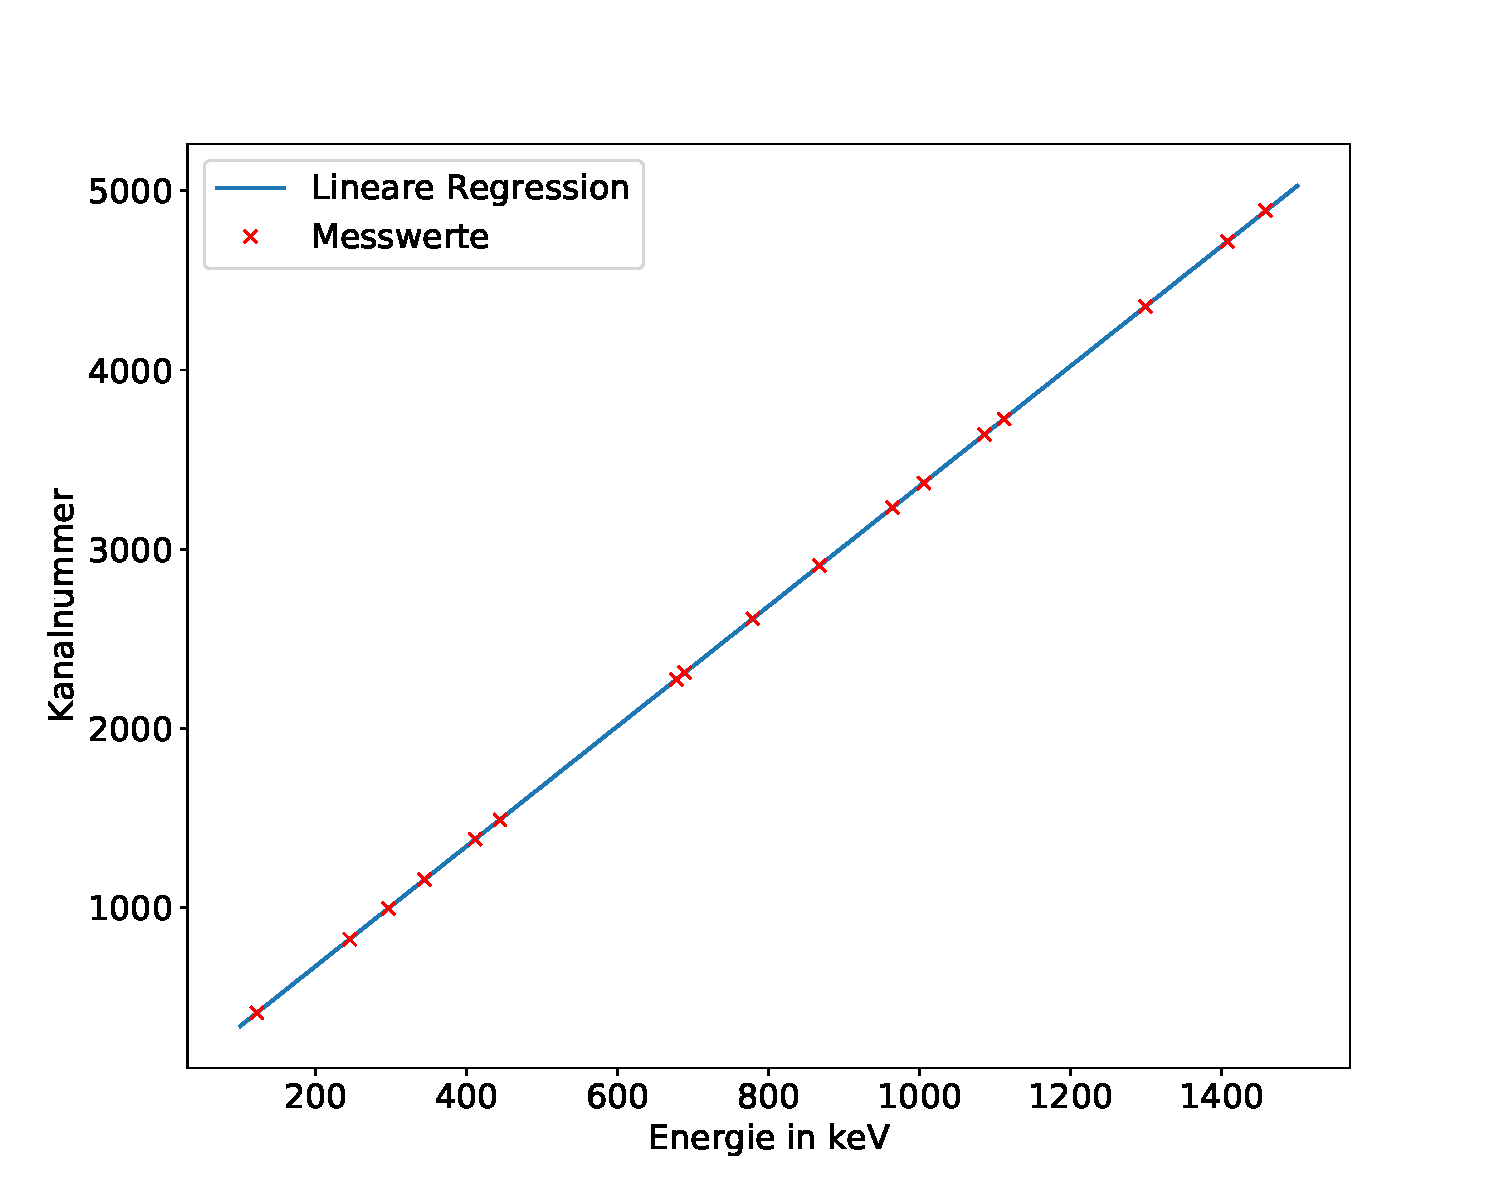
\includegraphics[width=0.7\textwidth]{python/plots/kalibrierung.pdf}
  \caption{Graphische Darstellung der linearen Fits an die Werte der Kalibrierungsmessung.}
  \label{fig:kalibrierung}
\end{figure}
\FloatBarrier
\subsection{Berechnung der Untergrundrate}
\label{subsec:a2}
Im Experiment wird immer dann ein Messwert aufgenommen, wenn auf ein Startsignal
innerhalb von der Suchzeit $T_\text{s} = \SI{20}{\micro\second}$ ein weiteres
Signal (Stopsignal) folgt. Für die Bestimmung der mittleren Lebenszeit der Myonen
sind nur die Fälle interessant, bei denen die Zeitmessung durch ein Myon-zerfall
induziertes Signal gestoppt wird. Da allerdings auch der Fall eintreten kann,
dass während der Suchzeit ein weiteres Myon in den Detektor einfällt und
die Zeitmessung stoppt. Diese Ereignisse werden im Folgenden als Untergrund bezeichnet.
Es wird davon ausgegangen, dass sich die Untergrundereignisse gleichmäßig auf
alle Kanäle verteilen, sodass eine konstante Untergrundrate zur Korrektur
von dem Inhalt jedes (nicht leeren) Bins abgezogen wird.\\ \\
Die Untergrundrate ergibt sich aus der Anzahl an Untergrundereignissen geteilt
durch die Zahl der gefüllten Kanäle ($342$).
Um die Zahl der Untergrundereignisse zu erhalten,
wird die Wahrscheinlichkeit dafür, dass innerhalb der Suchzeit $T_\text{s}$
genau ein einfallendes Myon im Detektor registriert wird, benötigt. Diese
Wahrscheinlichkeit folgt einer Poisson-Verteilung\cite{poisson}
\begin{equation}
  \label{eqn:poisson}
  p(n) = \frac{\mu^{n}}{n!} \cdot e^{-\mu}.
\end{equation}
Dabei bezeichnet $n$ die Anzahl gezählter Ereignisse und $\mu$ den
Erwartungswert.\\ Hier kann der Erwartungswert durch
\begin{equation}
  \label{eqn:erwartung}
  \mu = R \cdot T_\text{s}
\end{equation}
bestimmt werden. Wobei $R$ die Rate, mit der die Myonen in den Detektor einfallen,
angibt. Diese Einfall-Rate lässt sich widerum als
\begin{equation}
  \label{eqn:einfall}
  R = \frac{N_\text{start}}{t_\text{mess}},
\end{equation}
den gemessen Startsignalen $N_\text{start}$ pro Messzeit $t_\text{mess}$ ausdrücken.\\
Somit ergibt sich unter Verwendung der Gleichungen \eqref{eqn:poisson},
\eqref{eqn:erwartung} und \eqref{eqn:einfall}
eine Untergrundrate von\\ \\
\begin{align*}
  U =  \frac{p(1) \cdot N_\text{start}}{342} = \SI{3.549+-0.004}{} .
\end{align*}


\subsection{Experimentelle Bestimmung der mittleren Lebensdauer von Myonen}
\label{subsec:a3}
Zur Bestimmung der mittleren Myon-Lebensdauer wird an den in Abbildung \ref{fig:hist2}
dargestellten Messwerte eine lineare Regression der Gleichung \eqref{eqn:exp} entsprechenden Funktion
vorgenommen. Die Gewichtung stellt dabei der jeweilige Bininhalt dar. Dabei wird vor Durchführung der Regression, die in Abschnitt \ref{subsec:a2} berechnete
Untergrundrate $U$ von jedem Bin-Inhalt(ungleich $0$) abgezogen. Es ergibt sich die in Abbildung \ref{fig:hist2}
gezeigte Regressions-Funktion. In Abbildung \ref{fig:hist2_log} ist eine logarithmische Darstellung der y-Achse(counts) gewählt. Die Paramter der Regression lauten
\begin{align*}
  N_0 &= \SI{478.24+-14.61}{}\\
  \lambda &= \SI{472789.20+-20198.83}{\per\second} .
\end{align*}
Der Parameter $\lambda$ lässt sich als der Kehrwert der mittleren Lebensdauer identifizieren.\\
Somit beträgt die auf diese Weise experimentell ermittelte Lebendauer \\ \\
\begin{align*}
  \tau_{1} = \SI{2.12+-0.09}{\micro\second} .
\end{align*}
Die Abweichung zum Literaturwert \cite{lebensdauer}
\begin{align*}
  \tau_\text{literatur} = \SI{2.1969811+-0.0000022}{\micro\second}
\end{align*}
beträgt\\ \\
\begin{align*}
  \frac{\lvert \tau_\text{literatur} - \tau_{1} \rvert}{\tau_\text{literatur}} = \SI{4+-5}{\percent} .
\end{align*}
Eine andere Möglichkeit eine konstante Untergrundrate zu berücksichtigen, als die (analytische) Berechnung (siehe Abschnitt \ref{subsec:a2}),
ist den Untergrund als Paramter in der für die Regression verwendeten Funktion einzuführen. Dazu
wird Gleichung \eqref{eqn:exp} zu
\begin{equation}
  \label{eqn:exp_untergrund}
  N(t) = N_{0} \cdot e^{-\lambda \cdot t} + U
\end{equation}
abgeändert. Die Regression wurde in diesem Fall nur auf Messwerten, deren Counts ungleich $0$ sind, durchgeführt. Dies hat den Grund,
dass bei diesen Messwerten kein Untergrund vorliegen kann, da nichts gemessen wurde. Für die Regressions-Paramter ergeben sich
\begin{align*}
  N_{0} &= \SI{478.32+-14.58}{}\\
  \lambda &= \SI{469673.51+-25212.50}{\per\second}\\
  U &= \SI{2.71+-3.90}{}
\end{align*}
In Abbildung \ref{fig:hist} ist eine graphische Darstellung der Regression zu finden. In Abbildung \ref{fig:hist_log} ist eine logarithmische Darstellung der y-Achse(counts) gewählt.\\ \\
Damit ergibt sich eine mittlere Lebensdauer von\\ \\
\begin{align*}
  \tau_{2} = \SI{2.13+-0.11}{\micro\second} .
\end{align*}
Die Abweichung zum Literaturwert \cite{lebensdauer}
\begin{align*}
  \tau_\text{literatur} = \SI{2.1969811+-0.0000022}{\micro\second}
\end{align*}
beträgt\\ \\
\begin{align*}
  \frac{\lvert \tau_\text{literatur} - \tau_{2} \rvert}{\tau_\text{literatur}} = \SI{3+-5}{\percent} .
\end{align*}

\FloatBarrier
\begin{figure}
  \centering
  \includegraphics[width=1.2\textwidth]{python/plots/hist_u.pdf}
  \caption{Aufgenommes Histogramm der Zerfallszeiten(Counts abzüglich berechneter Untergrundrate), sowie Exponentieller-Fit.}
  \label{fig:hist2}
\end{figure}

\begin{figure}
  \centering
  \includegraphics[width=1.2\textwidth]{python/plots/hist_u_log.pdf}
  \caption{Aufgenommes Histogramm der Zerfallszeiten(Counts abzüglich berechneter Untergrundrate), sowie Fit der Messdaten (halblogarithmische Darstellung).}
  \label{fig:hist2_log}
\end{figure}

\begin{figure}
  \centering
  \includegraphics[width=1.2\textwidth]{python/plots/hist.pdf}
  \caption{Aufgenommes Histogramm der Zerfallszeiten, sowie Exponentieller-Fit(Untergrundrate als Parameter).}
  \label{fig:hist}
\end{figure}

\begin{figure}
  \centering
  \includegraphics[width=1.2\textwidth]{python/plots/hist_log.pdf}
  \caption{Aufgenommes Histogramm der Zerfallszeiten, sowie Exponentieller-Fit(Untergrundrate als Parameter, halblogarithmische Darstellung).}
  \label{fig:hist_log}
\end{figure}
\FloatBarrier
%\begin{figure}
%  \centering
%  \includegraphics{plot.pdf}
%  \caption{Plot.}
%  \label{fig:plot}
%\end{figure}
